\section{Architecture}

A program can be represented in several ways. There is extensive reading material on how logical programming can be used to represent and analyse programs\cite{Reps1995}\cite{DatalogDBQueries}. However, other approaches exist that lean more closely towards the implementation of our system.  As discussed in section \ref{subsec:staticAnalysis}, static analysis can be a means of representing implicit and explicit information about a piece of source code. For our approach, we needed a representation containing enough information to look up non-trivial properties about how information and data flows in the program. Abstract interpretation of a program produces an abstract state graph that meets these requirements. The graph contains information about control- and data flow, providing a rich source of information that can be extracted through some query language and a querying mechanism. 

% Querying mechanisms -> approaches in datalog queries enzo
Querying programs depends greatly on the way a program is represented and how queries are transformed into query-engine-friendly data structures. One way would be to resolve queries using existing techniques such as \cite{bddbddb}. This technique matches queries expressed in Datalog against a database of rules representing the relations of an entire program. Since our approach represents programs as flow graphs, an alternative method to resolve queries needs to be applied. A suitable algorithm to solving queries is presented in \cite{algoEngine}, which enables us to query flow graphs directly. The internals of this algorithm will be discussed in greater detail in section \ref{subsec:matchingEngine}.

% DSL
It is important that exploring and accessing information of a flow graph happens in an easy and user-friendly way. We believe regular path expressions to be the most legible way to write clean and understandable queries. With the JS-QL language, we offer an internal domain-specific language specialized in expressing queries corresponding to sequences of states in the flow graph. 

The actual architecture of the JS-QL framework is depicted in figure \ref{fig:architecture}. The query engine takes as input (i) a flow graph and (ii) a query, written in the JS-QL language. The output will consist of tuples \texttt{<State, Substitutions>} for all paths on which a match for the query was found.

\begin{figure}
    \centering
      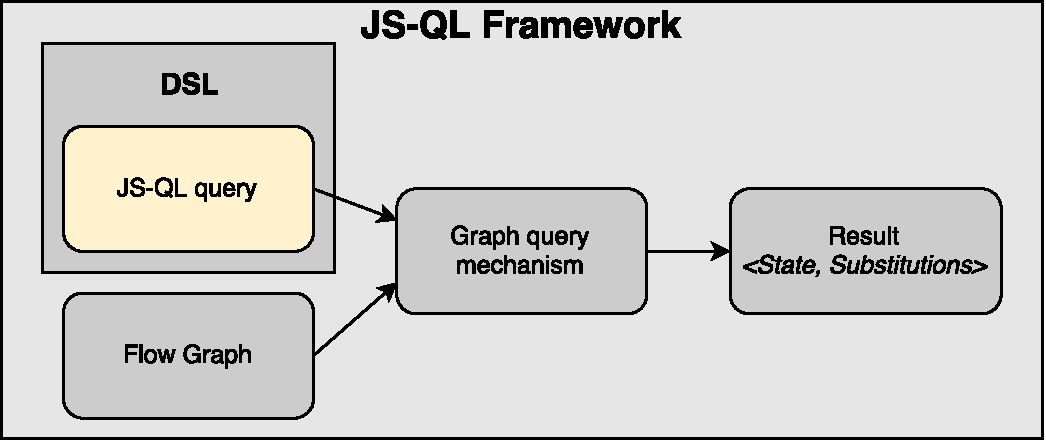
\includegraphics[width=0.9\textwidth]{images/Architecture} 
      \caption{JS-QL framework architecture}
    \label{fig:architecture}
\end{figure}
\section{Flow graphs for JavaScript programs}

The need for detailed control- and data flow information in our program representation graph limits the types of graphs that can be used for our framework. Program dependence graphs\cite{PDG} for example can be very useful to track the flow of information between certain points in a program but often lack more general information about program states, making them less qualified to use as our main program representation. In contrast, the JIPDA\cite{functionPurity} abstract state graph, generated by statically analyzing source code through \textit{abstract interpretation}, contains all the information needed to precisely express patterns to be detected in a program. This section takes an in-depth look at the JIPDA abstract state graph and the information it holds in its states. Figure \ref{fig:JipdaGraph} shows part of a typical graph produced by JIPDA for a program containing a check for whether a number is equal to zero or not.

As can be observed, the graph depicts all possible paths a program can traverse. Since the analysis in JIPDA is flow-sensitive, it is guaranteed that a state \texttt{a} on some path in the graph occurs before a state \texttt{b} on the same path if state \texttt{a} occurs first before state \texttt{b} on the path. This makes reasoning about patterns in a program much easier, since no false positives will occur with regards to the order of execution of states. The graph produced by the JIPDA analysis is also a flow graph, and more precisely maintains information about two types of flows:
%TODO uitleggen flow graph value flow en control flow -> in JIPDA

\begin{enumerate}
\item \textit{data flow}: Information about what values an expression may evaluate to.
\item \textit{Control flow}: Information about which functions can be applied at a call site.
\end{enumerate}

We need these kinds of information to be able to make correct assumptions at certain states in a program. Consider the expression \texttt{f(x)} for example. Function \texttt{f} will be the function that is invoked. The value of \texttt{f} however may depend on other operations that occur before this function call, such as another function call. Therefore it is important to know which function(s) \texttt{f} may refer to, illustrating the need of control and data flow.

\subsection*{States of an abstract state graph}

JIPDA internally uses Esprima\cite{Esprima} to parse JavaScript code and set up an abstract syntax tree (AST). This AST is the starting point for the analysis that JIPDA performs, hence information about the nodes from the AST is also contained in certain states in the resulting graph. The small-step semantics of a program are defined by an abstract machine that transitions between different states. The abstract machine is in eval-continuation style, indicating that a state is either an evaluation state or a continuation state. These states correspond to the states that can be seen in the abstract state graph. This graph is an alternation of four different types of states. These states are marked in red and are so-called \textit{evaluation states}. Other states are \textit{continuation states} (green), \textit{return states} (blue) and \textit{result states} (yellow). The states the machine can be in are described below:

\begin{figure}[!ht]
    \centering
      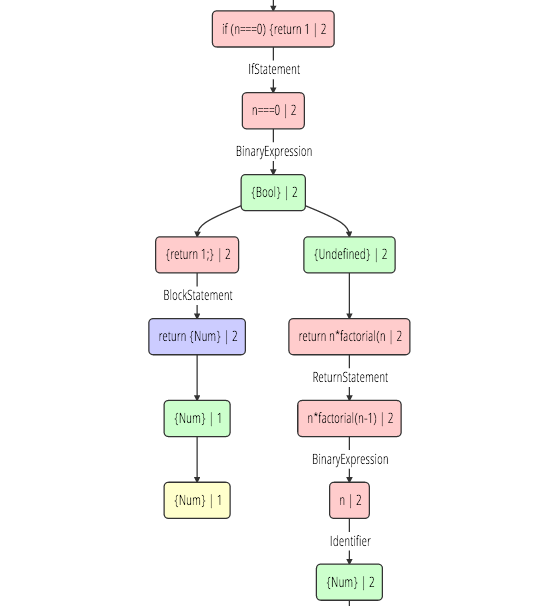
\includegraphics[width=262px, height=606px, keepaspectratio]{images/JipdaGraph} 
      \caption{Example JIPDA abstract state graph}
    \label{fig:JipdaGraph}
\end{figure}

%HELP VRAGEN BIJ JENS
\begin{enumerate}
\item \textit{Evaluation state}: Represents the evaluation of an expression of the program in the binding environment $\beta$.
\item \textit{Continuation state}: A state which indicates that the machine is ready to continue evaluation with the value it just calculated.
\item \textit{Return state}: This is a special kind of continuation state, as it indicates the return of a function application. When the machine is in this state it is ready to continue evaluation with the value calculated for the return of the function application.
\item \textit{Result state}: The final state of the graph, indicating the final computed value(s) of the program. This is also a special kind of continuation state. The machine and graph can have more than one result state, depending on the program's nature. 
\end{enumerate}

These states all contain valuable information about the point in the program they represent. The next part of this section discusses the different attributes that can be found in the states of the abstract state graph. 

%Kont, Lkont, Node, Benv, Store, Value
\subsection*{Node}

As said earlier, evaluation states contain information about the expression or statement they represent in the program. This information is stored in the form of an AST node, as obtained by the Esprima parser. Detailed information about the current expression or statement can be found in the properties of these nodes. Our approach makes extensive use of this information to find a match for a specified pattern along the graph. Note that node information is exclusively available in evaluation states. If we parse the following program \\\\
\texttt{function answerToTheUniverse(arg)\{}\\
\phantom{ }\phantom{ }\phantom{ }\phantom{ }\texttt{return 42;}\\
\texttt{\}}\\
\\
we obtain its corresponding JSON representation, listed in \ref{lst:EsprimaTree}.
\\
\begin{lstlisting}[label={lst:EsprimaTree},language=JSON,caption=Parsed JavaScript program AST, mathescape=true]  % float=t?

{
    "type": "Program",
    "body": [
        {
            "type": "FunctionDeclaration",
            "id": {
                "type": "Identifier",
                "name": "answerToTheUniverse"
            },
            "params": [
                {
                    "type": "Identifier",
                    "name": "arg"
                }
            ],
            "defaults": [],
            "body": {
                "type": "BlockStatement",
                "body": [
                    {
                        "type": "ReturnStatement",
                        "argument": {
                            "type": "Literal",
                            "value": 42,
                            "raw": "42"
                        }
                    }
                ]
            },
            "generator": false,
            "expression": false
        }
    ]
}
\end{lstlisting}

The parsed source code is a list of nodes contained in the body property of the "program" AST node. This is in fact the root node of the AST. Each node has its own \textit{type} that distinguishes different kinds of expressions and statements. The example code in \ref{lst:EsprimaTree} shows that the parsed code is a "FunctionDeclaration" with its own id, parameters, defaults and body attributes. We observe that the attributes in turn can again be (a list of) nodes.

\subsection*{Binding environment and store}

In JIPDA, variables point to addresses. The mapping of a variable to an address is called a \textit{binding}. These bindings reside in a \textit{binding environment} $\beta$. Each binding maps to a value through the \textit{store} $\sigma$. The store acts as a heap where bindings represent addresses on that heap. Being able to capture bindings, addresses and values in metavariables enables us to express and inspect data flow properties of programs. Variables are mapped to values in two stages. The first step for looking up a variable $\nu$ is to locate its binding in $\beta$. Next, the value of the variable can be looked up in the store by composing these two functions. The value of $\nu$ is given by $\sigma(\beta(\nu))$. This way of mapping variables to values allows us to reason about individual bindings, which is necessary because during interpretation multiple bindings to the same variable can exist simultaneously. Listing \ref{lst:benvStoreExample} gives an example of how a variable gets a binding and is later looked up.
\\
\begin{lstlisting}[label={lst:benvStoreExample},language=JavaScript,caption=Example of the binding environment and store workings, mathescape=true]  % float=t?

function f(){
  //$\beta$ contains a binding $x \rightarrow \widehat{Addr}$
  var x = 3; 
  
  //$\sigma$ has an entry $\widehat{Addr} \rightarrow \widehat{Val}$
  //and the (set of) corresponding value(s) for x is returned. 
  return x;
}
var value = f();
\end{lstlisting}


\subsection*{Value}
%Value uit store
The lookup of a variable through a binding in the store results in the (set of) value(s) for that variable. This information is available in all states but evaluation states. Values can either be addresses or undefined. For continuation states, the value will represent the looked up or calculated values of an expression. A return state's value is the set of possible values that will be returned. Result states contain the final values of a program.

\subsection*{Stack}

The stack is a local continuation delimited by a meta-continuation. The \textit{local continuation} is a (possibly empty) list of frames which acts as a stack (of frames), with normal push and pop functionalities. A \textit{meta-continuation} is either empty or a stack address pointing to the underlying stacks in the stack store. These stack addresses are generated at call sites and thus represent the application contexts. Useful information such as the call stack can be obtained by tracing out all reachable stack addresses in the stack store, starting from the context that is directly contained in the current state. The traversal of the stack terminates when we encounter an empty meta-continuation, also called the \textit{root context}. A program starts and terminates evaluation in this root context, provided that evaluation happens without errors. The root context corresponds to the top-level part of a program, the global namespace in JavaScript.

Although our framework doesn't provide stack traversal functionalities, basic properties of the stack (local continuation and meta-continuation) can be used and inspected to detect different kinds of states. For a function application, states corresponding with the start and end of the application will have the same local and meta-continuation. With this information, we can for example check for each path if there is a function application followed by a specific state \textit{before} the end of that function application. A concrete example of such a state is a recursive function call.

\section{External DSLs for querying graphs}

For almost any branch of science and engineering we can distinguish between two types of approaches. One type of approach is the \textit{generic} approach, which offers solutions to a wide range of problems within a certain domain. However, these solutions are often suboptimal. When we reduce the set of problems we want to solve, an often better approach to solving these problems would be the \textit{specific} approach.
In software engineering terms these two approaches translate to two types of languages: General purpose languages (GPLs) and domain-specific languages (DSLs) respectively. 
\textit{Domain-specific language} is no new concept. Many programming languages that are now considered general purpose language started out as domain-specific languages. Cobol, Fortran and Lisp for example all came into existence as dedicated languages for solving problems in a certain area\cite{vanDeursen:2000}, but gradually evolved into the full fledged languages they are today. The rest of this section is devoted to the comparison of GPLs and DSLs, in which we advocate that DSLs are the best approach for the instantiation of the JS-QL framework. We further give an overview of related work about DSLs for querying graphs.


\subsection{Domain-specific language vs. general purpose language}
\label{subsec:DSLvsGPL}

Before we start this comparison, we give a formal definition of domain-specific languages and general purpose languages:
\begin{definition}
    A \textit{domain-specific language} (DSL) is a programming language of executable specification language that offers, through approproate notations and abstractions, expressive power focused on, and usually restricted to, a particular problem domain.
\end{definition}

\begin{definition}
    A \textit{general purpose language} (GPL) is a programming language that is broadly applicable across application domains, and lacks specialized features for a particular domain.
\end{definition}

The key focus for DSLs are its focussed expressive power. The expressiveness of DSLs comes from the fact that they were created to solve a small set of problems. They offer a high-level set of mechanisms for the programmer to express his ideas for a particular application domain. A DSLs aim is to have the language focus specifically on those aspects and concepts that are relevant to a particular problem domain, hiding all boilerplate code that comes along with GPLs. Designers of general purpose programming languages also try to help the programmers express their ideas concisely and clear, but even with the most elegant programming language difficulties arise when programs get bigger and more complex. To this extent, extra features were developed for GPLs to further abstract code and reduce complexity. Amongst these features are functions, subroutines, packages, objects \dots  Even though these features are useful for general applications, the languages that implement them often have a set of operational baggage associated with them which makes a program unneccesarily complex to develop\cite{FluentInterfacesJava}. 

In contrast to the generic approach, the domain-specific approach to language design makes it possible to allow low-level system requirements to guide the design of the required high-level language features one wishes to incorporate into his language, instead of being required to use existing general-purpose designs.
We therefore believe that a domain-specific language is the best pick for our query language.
Benefits of domain-specific languages include:

%TODO: http://voelter.de/data/books/markusvoelter-dslengineering-1.0.pdf
\begin{itemize}
\item DSLs are application-specific. This allows users to express their ideas at the level of abstraction of the problem domain.
\item DSL programs are concise, self-documenting and highly reusable\cite{Bentley:1986}
\item Increased productivity: Once the language design and implementation have finished, work becomes much more efficient as you don't have to write the boilerplate code of the GPL manually. In this way you can replace a lot of GPL code with a few lines of DSL code.
\item Domain expert involvement: DSLs whose domain, abstractions and notations are closely aligned with how domain experts reason and express themselves, allow for a fluent integration between developers and domain experts. Domain experts can read, and possibly even write code in the language as they are not directly confronted with any implementation details.
\item Programs are often expressed at a level of abstraction that is meaningful for the domain. This brings along that these programs contain domain knowledge and that they can be reused with few to no modifications.
\item Improved code quality: Fewer bugs, better architectural conformance, increased maintainability. This is the result of the partially removing the programmers freedom and the avoidance of code duplication by providing DSL constructs.
\end{itemize}

\noindent Some counterarguments for using a DSL are:
\begin{itemize}
\item The cost of designing, implementing and maintaining a DSL
\item The cost of educating DSL users
\item A DSL has limited applicability
\item The difficulty of finding the correct scope for a DSL
\end{itemize}

We argue that the costs for setting up a DSL do not weigh up against the benefits of a DSL. The high reusability alone makes up for the one-time investment of designing and implementing the language. When developing a language for a certain domain, naturally its applicability will be limited to that domain only, as this is the purpose of a domain-specific language. Finding the correct scope for a DSL might be cumbersome, but there is a great amount of literature about specifying the domain of a problem\cite{Simos:1995} and the domain for DSLs\cite{karsai2014design}\cite{gunther2010agile}. 

\subsection{External DSLs}

Many DSLs come along with a compiler which translates DSL programs into applications. These kinds of DSLs are called \textit{external} DSLs. the compiler is also called an application generator\cite{Cleaveland:1988}, whereas the DSL is the application-specific language. The main advantage of external DSLs is that the implementation of the compiler can completely be tailored to the DSL. The DSL in turn is restricted in no way with regards to notation, primitives and the like because its syntax is independent of the underlying host language (since there is none). The remainder of this section discusses existing work about external DSLs used for graph traversal and graph querying.

\subsubsection*{StruQL}

StruQL is the query language behind the Strudel system\cite{Fernandez97aquery}. The language is built to support the retrieval and construction of data for web sites. This data is represented as \textit{data graphs} and originates from external sources, the integrated view and the web site itself. These data graphs depict web sites as nodes, representing web pages or atomic values, interconnected with directed, labelled edges. These edges then represent the links or attribute values that connect two nodes. The language enables users to create and query data graphs, but the real power of StruQL lies in their ability to express regular path expressions. This allows for very flexible queries describing the paths about which information needs to be accessed in great detail.
It also allows to compute the transitive closure of an \textit{arbitrary 2n-ary} relation, meaning that it can compute all reachable nodes from a certain node for any input graph. Buneman et al\cite{Buneman:1996} have formally proven that this is not a trivial computation.

\subsubsection*{GraphQL}
%http://sites.fas.harvard.edu/~cs265/papers/he-2008.pdf -> GraphQL

GraphQL\cite{He:2008} is a query language which allows to query graph databases. The language uses a graph pattern as a basic operational unit. These graph patterns consist of a graph structure and a predicate on attributes of the graph. They introduced the notion of formal languages for graphs. This is useful for composing and manipulating graph structures and is used as a basis of the graph query language.
The core of the language is a graph algebra in which the selection operator is generalized to graph pattern matching and a composition operator is introduced for rewriting matched graphs. In terms of expressive power, the language is contained in Datalog. This means that every query in GraphQL can be converted to a Datalog query. The language allows users to express concatenation, disjunction and recursion, allowing users to write dynamic queries. They address the NP-completeness of subgraph isomorphism by using neighborhood subgraphs and profiles, joint reduction of the search space, and optimization of the search order.

\subsubsection*{ASTLOG}
%http://www.cs.nyu.edu/~lharris/papers/crew.pdf
ASTLOG\cite{Crew:1997} is a query language for syntax-level C/C++ program analysis and is well suited to construct anchored patterns to match tree-like structures. The language is built as a Prolog variant syntax-wise, but instead of transforming an entire program into a database of Prolog rules, it is able to match \textit{objects} to queries directly. These objects are being made available through a C/C++ compiler frontend which provides an interface to the syntactic/semantic data structures build during the parse of a program. Among the available objects are the AST nodes of a program. These nodes can then be examined and queried by user-defined predicates in a similar fashion as one would do in Prolog. This allows for application-specific composable predicates. 

\subsubsection*{Lorel}
The Lorel language\cite{abiteboul1997lorel} was designed to query semistructured data. This kind of data can be seen as a graph with complex values at internal nodes, labeled edges and atomic leaves. The language's syntax resembles that of OQL (\textit{Object Query Language}), but has two two additional features: (i) A coercion mechanism for value/object comparisons and (ii) powerful path expressions. Coercion is needed for semistructured data, as two objects may represent the same data in different ways. Lorel introduces \textit{general path expressions}, a way to define label completion and regular expressions in paths. Regular expressions are supported through \texttt{.},\texttt{+},\texttt{?},\texttt{*},\texttt{()} and \texttt{|}, label completion is done as in SQL, namely with the \texttt{\%} symbol.
%http://infolab.stanford.edu/lore/pubs/lorel96.pdf -> Semistructured data

%-----------------------------
%RW over EDSL los van graphs:
%http://graphics.stanford.edu/hackliszt/liszt_sc2011.pdf
%http://homepages.cwi.nl/~jurgenv/papers/SCAM-2009.pdf
%https://www.researchgate.net/publication/220071161_BDL_A_Specialized_Language_for_Per-Object_Reactive_Control
%Chandra1999
%-----------------------------


\subsection{Internal DSLs}

In contrast to external DSLs, \textit{internal} (or \textit{embedded}\cite{Hudak:1996}) DSLs don't require a custom compiler. These languages inherit the infrastructure of some other (general purpose) language, and tailor it towards the domain of interest. In this way the language can be interpreted by its host language, saving the developer a lot of work. Although internal DSLs are restricted by the syntax of their host language, they can make full use of the host language as a sublanguage, thus offering the expressive power of the host language in addition to domain-specific expressive power of the DSL. This expressive power along with not having to build a fully fledged compiler for our DSL are the main reasons we prefer the internal DSL approach above the external DSL one. The rest of this section describes three internal DSLs, two for graph traversal and one that illustrates the flexibility and expressiveness of embedded DSLs. The terms internal DSL and embedded DSL both have the same meaning in the rest of this dissertation and both refer to the type of DSL that is embedded in a host language.

%Waarom internal
%----------------
%RW over DSEL graph traversal:
\subsubsection*{Gremlin}
%http://arxiv.org/pdf/1508.03843.pdf -> Graph traversal
\cite{Gremlin} presents the Gremlin graph traversal machine. The machine traverses graphs according to a user-specified traversal, making use of so-called traversers. These traversers can be seen as 'workers' who walk through the graph, keeping a bag of information on their back about the path they have already taken and the current graph node they are in. The machine is developed in such a way that it can be implemented as an embedded DSL in any host language, provided that the host language supports \textit{function composition} and \textit{functions functions as first-class entities}. The Gremlin language has an \textit{instruction set} of about 30 steps and each query is a sequence of these steps (i.e. a path). Querying graphs through paths is a well-known approach, but the Gremlin machine also supports nested paths for which each nested path is a graph traversal on it's own. Queries are transformed into traversals, so each traversal can be made application-specific. They present 9 different traversals, including a recursive and a domain-specific one. 

\subsubsection*{Dagoba}

Dagoba is an in-memory graph database system written in JavaScript. The chapter about Dagoba in the \textit{500 Lines or Less}\footnote{http://aosabook.org/en/500L} book provides an elaborate explanation on how to create a flexible, easily extensible internal DSL. The language is built as a fluent API, and explains which mechanics (such as lazy evaluation) go hand in hand with this kind of language representation. They also describe how they interpret the language and define some optimizations of the system, mainly through query transformators.

\subsubsection*{A little language for surveys}

A Little Language for Surveys \cite{RubyDSL} explores the use of the Ruby programming language to implement an internal domain-specific language. It checks how well the flexible and dynamic nature of the language accomodates for the implementation of a DSL for specifying and executing surveys. Two key features of the Ruby programming languages are exploited because they especially support defining internal DSLs: The flexibility of the syntax and the support for blocks. Function calls for example are easily readable, since the braces surrounding the arguments can be omitted and the arguments list can consist of a variable number of arguments (The latter is also supported in JavaScript\cite{Ecma6}). They make extensive use of the fact that entire blocks can be attached to method calls. These blocks are passed unevaluated to the called method, enabling \textit{deferred evaluation}. Next to these features, the meta-programming facilities of the Ruby makes it possible for them to read a DSL program and execute it in the contexts specified by that program. A two-pass architecture is used, splitting up the parsing and interpretation of the program. This is common practice for internal DSLs.

%Survey language -> illustrates flexibility of embedded dsl + design patterns
%
%-----------------------------
%RW over DSEL los van graphs:
%https://www.usenix.org/events/dsl99/full_papers/jennings/jennings.ps
%https://www.usenix.org/legacy/publications/library/proceedings/dsl97/full_papers/stevenson/stevenson.pdf
%http://haskell.cs.yale.edu/wp-content/uploads/2011/02/padl99.pdf
%Eliott1999
%https://www.usenix.org/legacy/publications/library/proceedings/dsl97/full_papers/kamin/kamin.pdf
%-----------------------------


\section{Design of an internal DSL for querying flow graphs}

%zie Domain-specific languages: An annotated Bibliography
Crafting a compiler for our languages falls outside the scope of this dissertation and we believe that the overhead for building an external DSL does not weigh up against the benefits of an internal DSL (as discussed in \ref{subsec:DSLvsGPL}).
In this section we discuss the design process of our internal domain-specific language named JS-QL.

\subsection{Internal DSL design constraints}

This section describe some factors that influenced the design of our query language. A first constraint for the language is that it was designed as an embedded DSL. This has as a consequence that we have to use the constructs and syntax the host language offers, JavaScript in our case. The JS-QL languages makes extensive use of JavaScript \texttt{Object}s that function as dictionaries. A limitation for us was that these dictionaries only accept strings as keys. Function calls for example can't serve as keys in JavaScript objects as their value can't always be calculated at compile time. This was a serious drawback for us and it even lead to an inconsistency in our language, as will be discussed in chapter \ref{ch:JSQL}. 
Our language has to be easily extensible as users need to be able to specify their own predicates and policies. To this extent, JavaScript surfaced as an ideal language. The dynamic typing and optional function arguments made creating flexible predicates and policies a lot easier.

Flow graphs need to be queried, so the language has to fit these needs in the form of appropriate predicates. The design of our language depended on the information that is contained in each state of the graph. The JIPDA graph states contain several fields that in turn can recursively contain other fields. The nature of the algorithm we use together with the structure of these states asked for a close mapping of states to query predicates. As JavaScript objects are great for storing nested information, we chose to use them as a mapping for states. From now on these objects will be referred to as \textit{dictionaries}. Fields in a dictionary now have a one-to-one relationship with fields in a state, making the matching process for the algorithm less of a burden. Another constraint imposed by the flow graph was that sequences of states had to be expressed in a precise yet legible fashion. This had as a result that the language was set up as a fluent interface, enabling the user to specify a number of states separated with a simple dot. We can thus say that the type of graph helped shape the JS-QL language.

%GEEN REPL
A final constraint was the need of an environment where queries can be expressed and evaluated against the flow graph. It would be tiresome to specify queries in one place and the input program elsewhere. This would also imply that every time a change to the program or the query has to be made, at least one separate file has to be modified. This is clearly not an optimal solution. As there is no \textbf{r}ead \textbf{e}val \textbf{p}rint \textbf{l}oop (REPL) available for JavaScript in the browser, we opted to extend the existing environment of the JIPDA analysis with support for (i) writing queries and (ii) checking these queries against the flow graph.


\subsection{DSL implementation techniques and patterns}

\begin{figure}[!h]
    \centering
      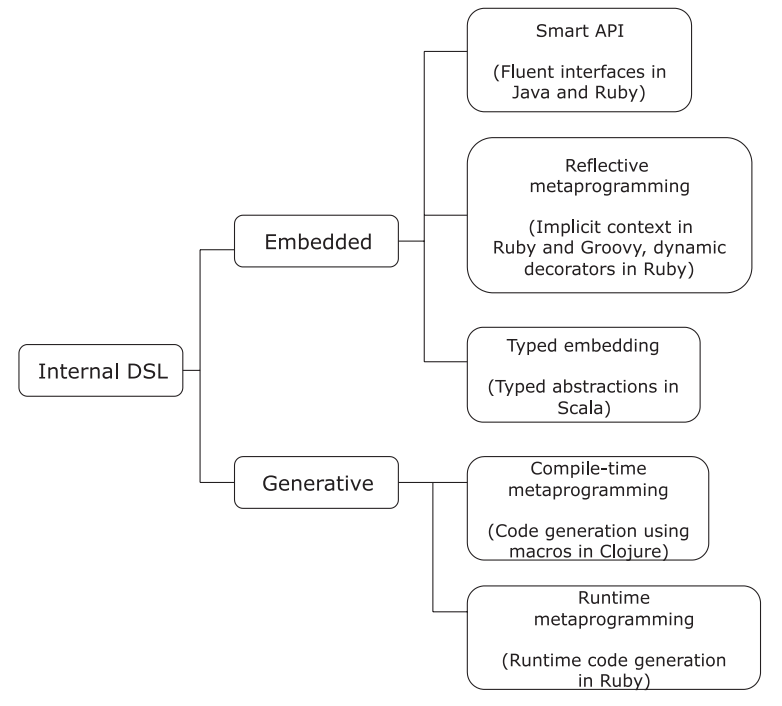
\includegraphics[width=0.8\textwidth]{images/DSLTechniques} 
      \caption{Internal DSL implementation techniques}
    \label{fig:DSLTechniques}
\end{figure}

Figure \ref{fig:DSLTechniques} shows the different kinds of implementation techniques for internal DSLs, as specified by \cite{Ghosh:2010}. Our DSL doesn't generate any code, so we won't discuss generative internal DSLs. Embedded internal DSLs on the other hand can be implemented in three ways: 

\begin{enumerate}
\item \textit{Smart API}: Readability is key for DSLs. Implementing a fluent interface is a way to improve readability and make Smart APIs. To this extend method chaining is a popular technique: It can be implemented by making the output of one method flow naturally as the input of another. Benefits are that a series of invocations in the DSL feel more natural and that it expresses the series of actions you want to perform or detect in the problem domain. Boilerplate code is not needed for this type of internal DSL, hence the name \textit{Smart} API.
\item \textit{Reflective metaprogramming}: The decorator pattern\footnote{https://en.wikipedia.org/wiki/Decorator\_pattern} is a well known pattern for extending individual objects. The ability to extend individual objects in a DSL greatly adds flexibility to the language. For some dynamically typed programming languages it is possible to define dynamic builders. These builders have a similar objective as the decorator pattern: construct an object incrementally within a DSL. This technique allows the language designer to smooth out the implementation aspect of the DSL by letting the user construct methods dynamically through the meta-object protocom of the language runtime.
\item \textit{Type embedding}: Types make for more concise and robust code. This is the philosophy that is behind the type embedding technique. Internal DSLs with a statically typed host language often use this pattern to make the language more expressive using the power of a type system. Each abstraction in the domain model should be made typed (and generic). This allows for fewer code duplication and a large part of the work will be done by the compiler of the host language. By making abstractions typed, correctness of programs written in the DSL is guaranteed: If the code compiles, it will most likely be correct.
\end{enumerate}

For our internal language we can already rule out the type embedding technique as JavaScript is a dynamically typed language. The problem domain of our approach doesn't need extra functionality to be added to individual objects in our language. These individual objects in our case are the states of the flow graph. States already are self-contained (they contain all necessary information) and don't require additional individual functionality. 

This leaves us with the smart API approach, which is ideal for our domain. By chaining methods in our DSL we can specify which states we want to encounter along the graph in a clearly specified order. Combining a smart API with several carefully chosen DSL design patterns\cite{DSLFowler} result in the concise and easily readable language that JS-QL is today. The remainder of this section elaborates on the chosen design patterns.

\subsubsection*{Method chaining}

Method chaining is the bread and butter of our DSL and at the same time also the \textit{only} way of expressing queries. This approach offers a fluent interface to the user in which it is hard to make any coding mistakes. The ability to express a state one wishes to encounter as a chained method to states he discovered earlier in the graph allows to build very readable queries. We illustrate this with an example: \texttt{G.skipZeroOrMore().functionCall()}. It is immediately obvious that this code is very intuitive: \texttt{G} is the entry point of our language, which indicates the start of a query. We then search for a path in the graph that contains a function call somewhere down that path. This is expressed by \texttt{skip}ping some, possibly none, states until a function call state is encountered.

\subsubsection*{Literal map}
%literal map
%-> Argument is a map similar to literal map
Specifying that one wishes to find states is often quite general. To this extent we need some sort of mechanism to express which types of states we want to match and what information we want to capture in (meta)variables. A literal map provides just this functionality by letting the user specify detailed key-value pairs. An example for could be: \texttt{.functionCall({name: 'f', arguments: '?args'})}. The literal map, enclosed in curly braces, indicates that only fuction calls with name \texttt{f} need to be matched and that the arguments of the matched state need to be captured in metavariable \texttt{?args}.

\subsubsection*{Object scoping}

The example for the method chaining design pattern is also applicable for the object scoping pattern. A single entry point \texttt{G} is created for queries, limiting the impact of the query that object. This pattern remedies two JavaScript flaws: Global namespace pollution and malicious code injection. This malicious code will only harm the \texttt{G} object, which is contained in some sort of sandbox.
%object scoping
%-> Alles wordt geevalueerd tegen 1 object om global namespace pollution tegen te gaan (alsook security issues)

\subsubsection*{Deferred evaluation}
%deferred evaluation
%-> Used to specify extra properties (not available at compile-time) + filters on values that aren't available
Some queries contain definitions for extra properties and filters. The information for these filters and properties is often not available at compile-time of our language. A mechanism is needed to delay the evaluation of those filters and properties until the matching process in the backend has collected enough information. Our framework handles this by creating thunks for filters and properties and unwrapping these thunks when the matching engine needs to evaluate them. By the time the evaluation happens, all variables should be bound in these thunks in previous matching steps. Consider a metavariable \texttt{?val} which captures the value of an assignment. If we only want to match assignment states with a value greater than 2, we have to create a thunk for the filter function \texttt{>} with arguments \texttt{?val} and \texttt{2}. We can't disregard states with \texttt{?val} greater than 2 immediately, as we don't know which value will be bound to \texttt{?val} at compile time.

\subsubsection*{Delimiter directed translation}
%delimiter directed translation
%-> Every method call is evaluated/parsed separately
Inherent to our DSL is delimiter directed translation. As method chaining is used as a means to set up our fluent interface, all methods are separated by a dot (the delimiter). Each method separated by this dot gets separately translated internally into a representation that is easier for our backend to process.

\subsubsection*{Newline separators}

Finally, the newline separators design pattern is incorporated in our DSL. This design pattern allows users to enter newlines between parts of their code. This greatly improves the readability and can split a program up in logical parts. Our DSL supports newlines in queries. This can be very useful to separate different states or sequences of states. Consider an example in which we only want to find assignments to variables \texttt{a} and \texttt{b}. Code can then be divided in two distinct parts, as in example \ref{lst:newlineSeparators}.

\begin{lstlisting}[label={lst:newlineSeparators},language=JavaScript,caption=Newline separators,mathescape=true]  % float=t?

.assign({leftName: 'a'}) //first logical part
.or()
.assign({leftName: 'b'}) //second logical part
\end{lstlisting}
%newline separators
%-> Language supports newlines between every state


